\documentclass[12pt, a4paper]{article}
\usepackage[UTF8]{ctex}
\usepackage{amsmath}
\usepackage{amssymb}
\usepackage{amsthm}
\usepackage{geometry}
\usepackage{enumitem}
\usepackage{indentfirst}
\usepackage{caption}
\usepackage{fancyhdr}
\usepackage{booktabs}
\usepackage{titlesec}
\usepackage{draftwatermark}
\usepackage{graphicx} % 导入图像的宏包、单图




% 页面布局设置
\geometry{top=2.54cm, bottom=2.54cm, left=3.18cm, right=3.18cm}

% 行距设置
\linespread{1.5}

%设置水印
\SetWatermarkText{B站：布加拉提}
\SetWatermarkScale{0.4}
% 段落设置
\setlength{\parindent}{2em}
\setlength{\parskip}{0.5em}

% 节标题格式设置
\titleformat{\section}{\normalfont\Large\bfseries}{第\chinese{section}章、}{1em}{}
\titlespacing{\section}{0pt}{2.5ex plus 1ex minus .2ex}{1.3ex plus .2ex}

% 定理环境设置
\newtheoremstyle{solution}
{}
{}
{}
{}
{\bfseries}
{、}
{1em}
{}
\theoremstyle{solution}
\newtheorem{sol}{解}

% 页眉页脚设置
\pagestyle{fancy}
\fancyhf{}
\fancyhead[C]{b站布加拉提整理（回忆版）b站甘茶w独家讲解}
\fancyfoot[C]{\thepage}

\rfoot{整理人：八方\\资源提供：考研乔瑟夫}
\lhead{
\includegraphics[width=0.06\linewidth]{p1.png}}
\rhead{
\includegraphics[width=0.06\linewidth]{p2.png}}
\renewcommand{\headrulewidth}{0.4pt}
\renewcommand{\footrulewidth}{0.4pt}

\begin{document}

\begin{center}
\Large\textbf{2008哈工大硕士考试试题：805物理光学}
\end{center}




\section*{一、填空与选择（28分）}
\begin{enumerate}
    \item \_\_\_\_\_称为波面。
    \item 发生全发射的条件是\_\_\_\_\_，全反射现象的特点是\_\_\_\_\_，\_\_\_\_\_，\_\_\_\_\_。
    \item 两个频率相同、振动方向相同，而转播方向相反的单色光波叠加产生\_\_\_\_\_，相邻两个波节之间的距离为\_\_\_\_\_。
    \item 椭圆偏振光分为\_\_\_\_\_和\_\_\_\_\_两种。
    \item 在相干照明的情况下，平行平板的产生\_\_\_\_\_，楔形平板产生成\_\_\_\_\_干涉。
    \item 产生干涉的条件是光波\_\_\_\_\_，\_\_\_\_\_，\_\_\_\_\_。
    \item 根据瑞利判据，望远镜的分辨率为\_\_\_\_\_，照相机物镜的分辨率为\_\_\_\_\_，显微镜的分辨率为\_\_\_\_\_。
    \item 在真空中传播的平面电磁波，其电场表达式为$E_x=0,E_y=0,E_z=(10^2V/m)cos[\pi\times10^{14}s^{-1}(t-x/c)+\pi/2]$,该电磁波的频率，波长为\_\_\_\_\_，周期为\_\_\_\_\_，振幅为\_\_\_\_\_，初相位为\_\_\_\_\_.
    \item 在\_\_\_\_\_情况，在光波介质面上只发生折射，没有反射光。
    \item （重复）使自然光相继通过三个偏振片，第一个与第三个偏振片的透光轴（从偏振光透出的偏振光的振动方向）正交，第二个偏振片的透光轴与第一个偏振片的透光轴成$30^\circ$角，若入射自然光的强度为$I_0$，则最后透出的光强为\_\_\_\_\_。
\end{enumerate}
\section*{二、解释下列名词（30分）}
\begin{enumerate}
    \item 色散
    \item 半波损失
    \item 艾里斑
    \item 群速度
    \item 双折射
    \item 巴比涅原理
    \item 磁光效应
    \item 古斯——哈斯恩位移
\end{enumerate}
\section*{三、简答题}
\begin{enumerate}       
    \item 比较等倾圆条纹与牛顿环条纹的异同。
    \item 简述利用单个光源获取相干光的方法，并列举干涉装置。
    \item 光波在金属反射与在玻璃表面反射相比，其反射波有什么特点？
    \item 影响干涉条纹对比度的因素有哪些？
    \item 简答光波在各项同性介质和各向异性介质中的传播时，有何不同？
\end{enumerate}
\section*{四、计算与论述}
\begin{enumerate} 
    \item 纳黄光包含589.6$nm$和589.0$nm$两种波长，要在光波的一级光谱中分辨开这两种波长的谱线，光栅至少应该有多少条缝？
    \item 夜间，在一棵人造卫星拍地球的照片。如果所用照相机镜头的焦距为50$mm$,$F$数为2，试问在100$km$以外能否分辨开汽车上的两盏灯（假定车灯间距为1000$mm$）?
    \item 如图所示，以知一束自然光入射到折射率$n=4/3$的水面上时反射光是偏振的。一块折射率$n=1.5$的平面玻璃浸在水下，若要使玻璃表面的反射光$o'n'$也是线偏振的，求玻璃表面与水平面夹角$\alpha $应该为多大？
        \begin{figure}[!htb]
        \centering
        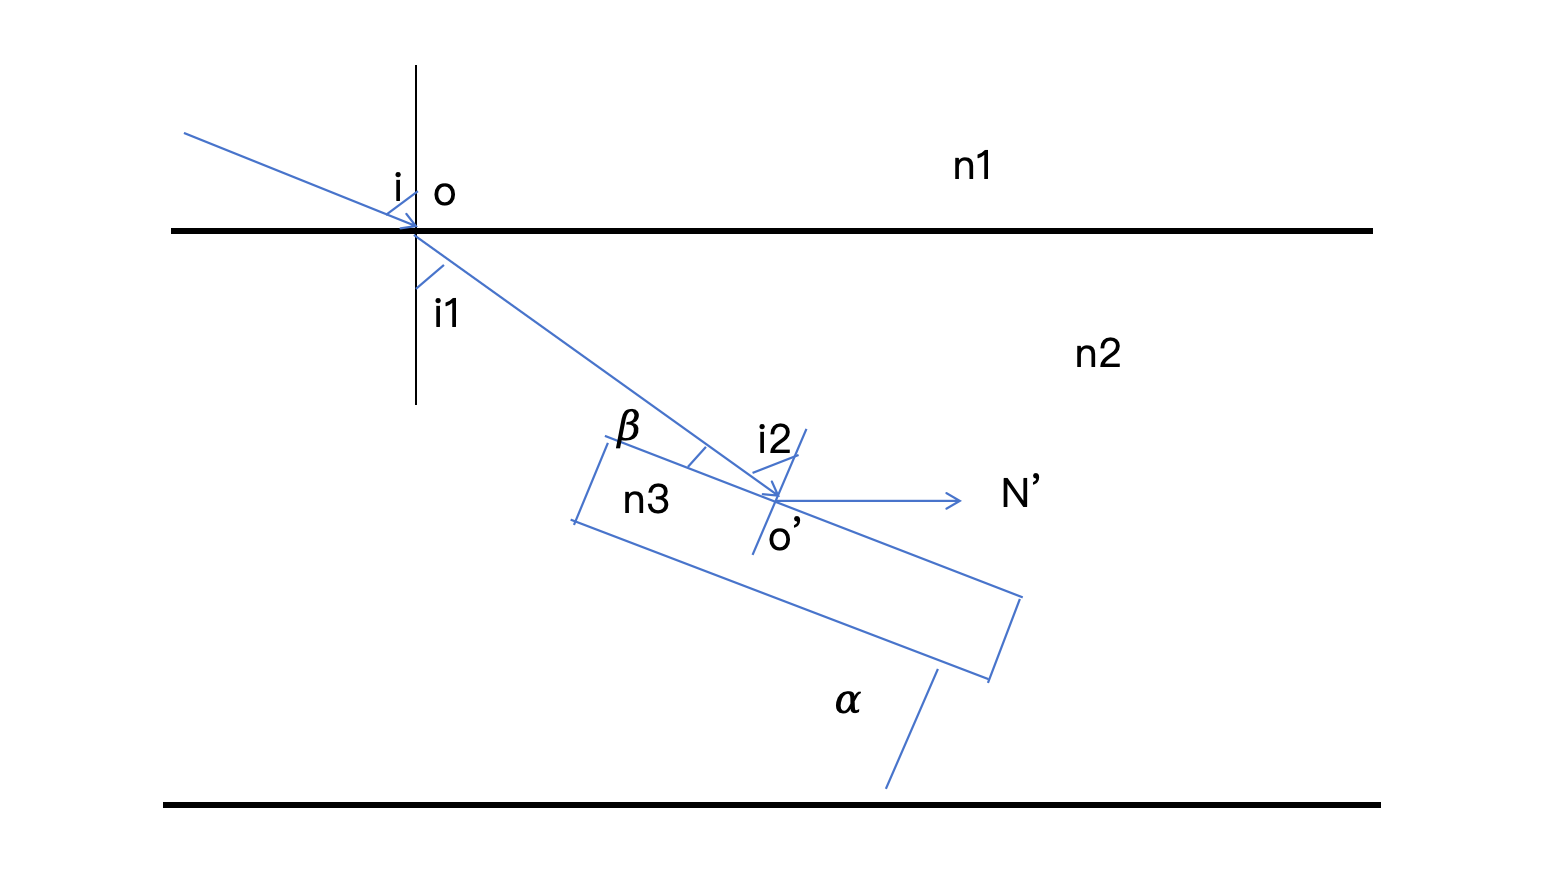
\includegraphics[width=0.5\linewidth]{08.png}
    \end{figure}
    \item 一种光栅的结构是将平行光束衍射到它自身的相反方向，试问：
        \begin{enumerate}
            \item 如果该光栅每单位长度上有八条线，什么样的波长将以入射角$\theta$方向衍射？（$\theta$是光法线和入射方向之间的夹角）
            \item 如果有两种波长$\lambda_1,\lambda_2$的光入射，能否用这种结构的光栅能否将此光束单色化？为什么？
        \end{enumerate} 
    \item 画出马赫-泽德干涉仪原理，当光源分别为点光源和拓展光源时，讨论干涉条纹的定域性。
\end{enumerate}
\end{document}

